% Figure per il Capitolo 2 - Threat Landscape e Sicurezza Distribuita
% Da inserire nel documento LaTeX principale

% Preambolo necessario (se non già presente):
\usepackage{tikz}
\usepackage{pgfplots}
\usetikzlibrary{arrows.meta, positioning, shapes, shadows, patterns, decorations.pathreplacing}
\pgfplotsset{compat=1.17}

% FIGURA 2.1: Amplificazione Non-Lineare della Superficie di Attacco
\begin{figure}[htbp]
\centering
\begin{tikzpicture}
\begin{axis}[
    width=12cm,
    height=8cm,
    xlabel={Numero di Punti Vendita},
    ylabel={Fattore di Amplificazione ASSA},
    xmin=0, xmax=550,
    ymin=0, ymax=14,
    xtick={0,50,100,200,300,400,500},
    ytick={0,2,4,6,8,10,12,14},
    grid=both,
    grid style={line width=.1pt, draw=gray!20},
    major grid style={line width=.2pt,draw=gray!50},
    legend pos=north west,
    legend style={font=\footnotesize}
]

% Dati dalla simulazione
\addplot[
    color=blue,
    mark=*,
    line width=1.5pt,
    mark size=3pt
] coordinates {
    (0,1)
    (50,2.3)
    (100,3.8)
    (200,6.2)
    (300,8.4)
    (400,10.1)
    (500,11.7)
};
\addlegendentry{ASSA Osservato}

% Fit polinomiale
\addplot[
    color=red,
    dashed,
    line width=1.2pt,
    domain=0:550,
    samples=100
] {1 + 0.035*x + 0.00004*x^2};
\addlegendentry{Fit Polinomiale}

% Area di confidenza
\addplot[
    name path=upper,
    draw=none,
    domain=0:550,
    samples=50
] {1 + 0.035*x + 0.00004*x^2 + 0.5};

\addplot[
    name path=lower,
    draw=none,
    domain=0:550,
    samples=50
] {1 + 0.035*x + 0.00004*x^2 - 0.5};

\addplot[gray!20, opacity=0.5] fill between[of=upper and lower];

% Annotazioni
\node[anchor=west] at (axis cs:250,10) {\footnotesize Crescita super-lineare};
\draw[<-,thick] (axis cs:200,6.2) -- (axis cs:180,7.5);

\end{axis}
\end{tikzpicture}
\caption{Amplificazione Non-Lineare della Superficie di Attacco con Scala della Rete. L'ASSA cresce in modo super-lineare con il numero di punti vendita a causa delle interconnessioni crescenti e dei percorsi di propagazione multipli.}
\label{fig:assa-amplification}
\end{figure}

% FIGURA 2.2: Evoluzione del Threat Landscape GDO 2020-2025
\begin{figure}[htbp]
\centering
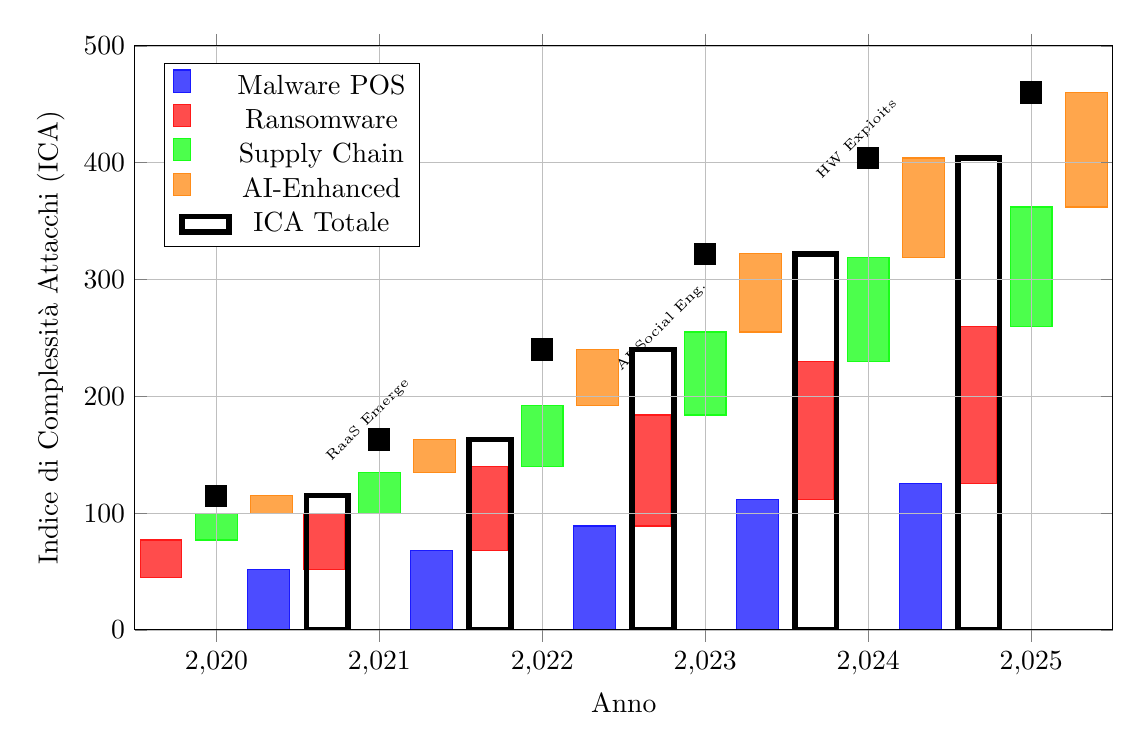
\begin{tikzpicture}
\begin{axis}[
    width=14cm,
    height=9cm,
    xlabel={Anno},
    ylabel={Indice di Complessità Attacchi (ICA)},
    xmin=2019.5, xmax=2025.5,
    ymin=0, ymax=500,
    xtick={2020,2021,2022,2023,2024,2025},
    ytick={0,100,200,300,400,500},
    grid=both,
    grid style={line width=.1pt, draw=gray!20},
    major grid style={line width=.2pt,draw=gray!50},
    legend pos=north west,
    ybar=5pt,
    bar width=15pt,
    area style,
]

% Barre per categorie di attacco
\addplot[ybar stacked, fill=blue!70, draw=blue!90] 
    coordinates {
        (2020,45) (2021,52) (2022,68) (2023,89) (2024,112) (2025,125)
    };
\addlegendentry{Malware POS}

\addplot[ybar stacked, fill=red!70, draw=red!90] 
    coordinates {
        (2020,32) (2021,48) (2022,72) (2023,95) (2024,118) (2025,135)
    };
\addlegendentry{Ransomware}

\addplot[ybar stacked, fill=green!70, draw=green!90] 
    coordinates {
        (2020,23) (2021,35) (2022,52) (2023,71) (2024,89) (2025,102)
    };
\addlegendentry{Supply Chain}

\addplot[ybar stacked, fill=orange!70, draw=orange!90] 
    coordinates {
        (2020,15) (2021,28) (2022,48) (2023,67) (2024,85) (2025,98)
    };
\addlegendentry{AI-Enhanced}

% Linea di trend totale
\addplot[
    color=black,
    mark=square*,
    line width=2pt,
    mark size=3pt
] coordinates {
    (2020,115) (2021,163) (2022,240) (2023,322) (2024,404) (2025,460)
};
\addlegendentry{ICA Totale}

% Eventi chiave
\node[anchor=south, rotate=45, font=\tiny] at (axis cs:2021,170) {RaaS Emerge};
\node[anchor=south, rotate=45, font=\tiny] at (axis cs:2022.8,250) {AI Social Eng.};
\node[anchor=south, rotate=45, font=\tiny] at (axis cs:2024,410) {HW Exploits};

\end{axis}
\end{tikzpicture}
\caption{Evoluzione del Threat Landscape GDO 2020-2025. L'ICA mostra una crescita del 312\% nel periodo, con accelerazioni correlate all'introduzione di nuove tecnologie di attacco.}
\label{fig:threat-evolution}
\end{figure}

% FIGURA 2.5: Framework Integrato di Sicurezza GDO
\begin{figure}[htbp]
\centering
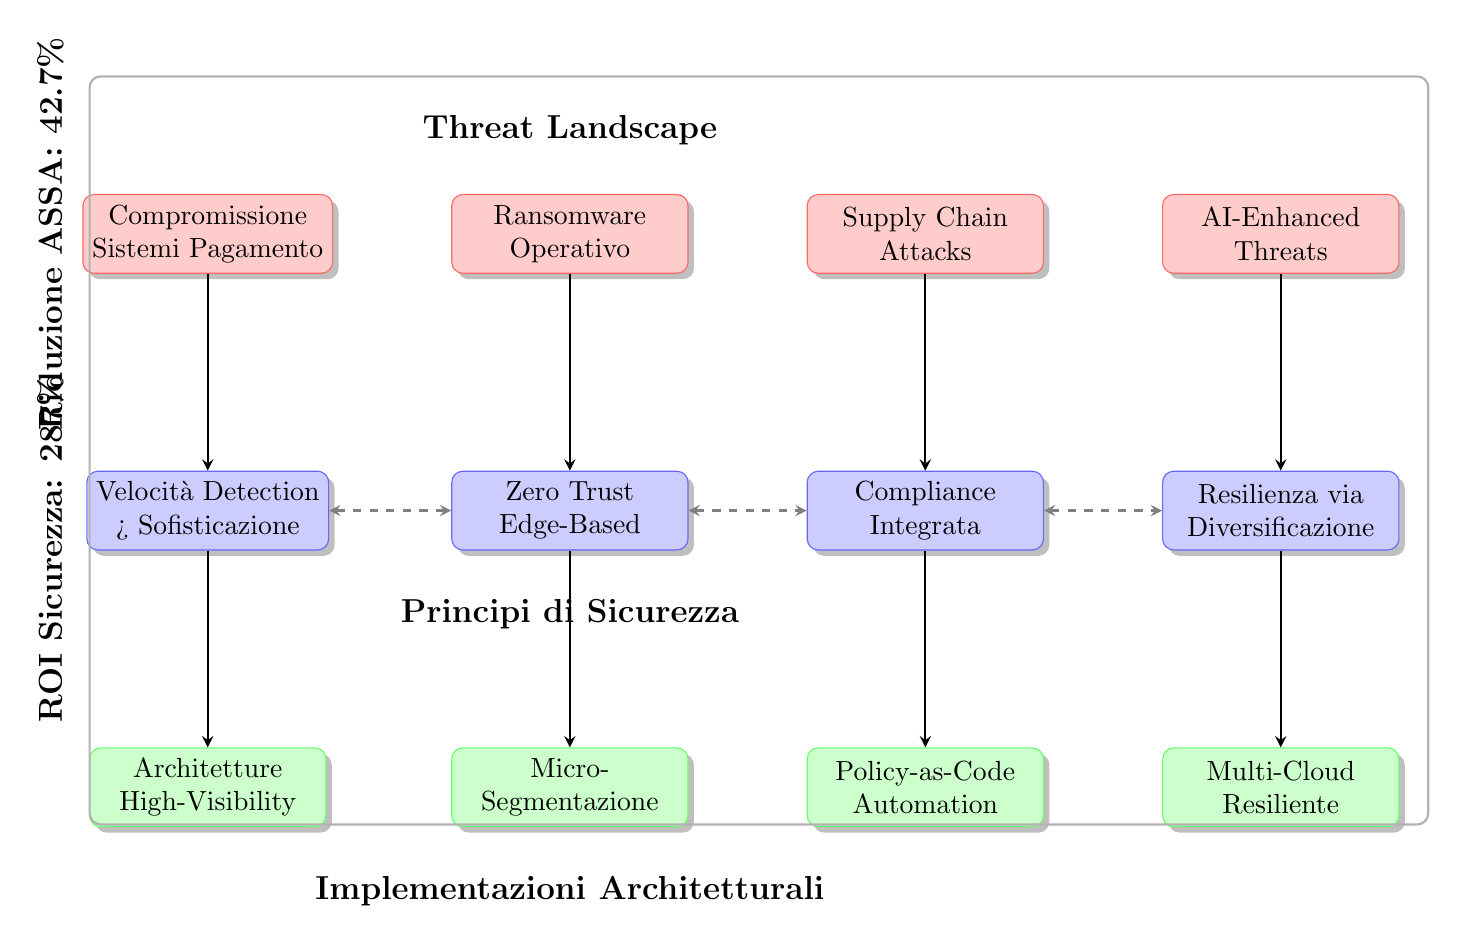
\begin{tikzpicture}[
    node distance=1.5cm,
    box/.style={rectangle, draw, rounded corners, minimum width=3cm, minimum height=1cm, align=center, fill=white, drop shadow},
    threat/.style={box, fill=red!20, draw=red!60},
    principle/.style={box, fill=blue!20, draw=blue!60},
    architecture/.style={box, fill=green!20, draw=green!60},
    arrow/.style={->, >=stealth, thick},
    doublearrow/.style={<->, >=stealth, thick}
]

% Threat Landscape Layer
\node[threat] (pos) {Compromissione\\Sistemi Pagamento};
\node[threat, right=of pos] (ransomware) {Ransomware\\Operativo};
\node[threat, right=of ransomware] (supply) {Supply Chain\\Attacks};
\node[threat, right=of supply] (ai) {AI-Enhanced\\Threats};

\node[above=0.5cm of ransomware, font=\large\bfseries] {Threat Landscape};

% Principi Emergenti Layer
\node[principle, below=2.5cm of pos] (detection) {Velocità Detection\\> Sofisticazione};
\node[principle, below=2.5cm of ransomware] (zerotrust) {Zero Trust\\Edge-Based};
\node[principle, below=2.5cm of supply] (compliance) {Compliance\\Integrata};
\node[principle, below=2.5cm of ai] (resilience) {Resilienza via\\Diversificazione};

\node[below=0.5cm of zerotrust, font=\large\bfseries] {Principi di Sicurezza};

% Implicazioni Architetturali Layer
\node[architecture, below=2.5cm of detection] (visibility) {Architetture\\High-Visibility};
\node[architecture, below=2.5cm of zerotrust] (microseg) {Micro-\\Segmentazione};
\node[architecture, below=2.5cm of compliance] (automation) {Policy-as-Code\\Automation};
\node[architecture, below=2.5cm of resilience] (multicloud) {Multi-Cloud\\Resiliente};

\node[below=0.5cm of microseg, font=\large\bfseries] {Implementazioni Architetturali};

% Connessioni verticali
\foreach \source/\dest in {pos/detection, ransomware/zerotrust, supply/compliance, ai/resilience,
                          detection/visibility, zerotrust/microseg, compliance/automation, resilience/multicloud} {
    \draw[arrow] (\source) -- (\dest);
}

% Connessioni orizzontali (interdipendenze)
\draw[doublearrow, dashed, gray] (detection) -- (zerotrust);
\draw[doublearrow, dashed, gray] (zerotrust) -- (compliance);
\draw[doublearrow, dashed, gray] (compliance) -- (resilience);

% Box contenitore
\draw[thick, rounded corners, draw=gray!60] (-1.5,-7.5) rectangle (15.5,2);

% Metriche sul lato
\node[rotate=90, anchor=center] at (-2,0) {\large\bfseries Riduzione ASSA: 42.7\%};
\node[rotate=90, anchor=center] at (-2,-4) {\large\bfseries ROI Sicurezza: 287\%};

\end{tikzpicture}
\caption{Framework Integrato di Sicurezza GDO. Il diagramma mostra la relazione causale tra threat landscape, principi di sicurezza emergenti e implementazioni architetturali concrete, con le metriche di impatto risultanti.}
\label{fig:security-framework}
\end{figure}